$subject$=Физические основы компьютерных \\ и сетевых технологий
$teacher$=Лекции Герта А. В.
$date$=10.02.2025

\section{Лекция 1. Магнитное поле}

Давным-давно верили, что существовал \enquote{эфир}, который опоясывал всю вселенную и который был посредником в гравитационных/электромагнитных 
взаимодействиях. Позднее от теории эфира перешли к теории поля. Согласно нее каждый электрический заряд создает электрическое поле, 
которое действует на другие заряды

Опыт показывает, что сила $\vec{F}$, действующая на точечный заряд $q$, зависит в общем случае не только от положения этого \
заряда, но и от его скорости $v$. Соответственно этому силу $F$ разделяют на две составляющие - электрическую $F_\text{Э}$ 
(не зависит от движения заряда) и магнитую $F_\text{М}$ (зависит от скорости заряда). В любой точке пространства направление и модуль
магнитной силы зависят от скорости $v$ заряда, причем эта сила всегда перпендикулярна вектору $v$. Свойства магнитной 
силы можно описать, если ввести понятие магнитного поля. Силовой характеристикой магнитного поля (его действия на двигающиеся заряженные частицы)
в данной точке пространства является вектор магнитной индукции $B$. Он определяет магнитную силу, действующую на двигающийся электрический заряд $q$

\[F_\text{М} = q [\vec{v}, \vec{B}]\]

Полная электромагнитная сила, действующая на заряд $q$: $F_L = q\vec{E} + q[\vec{v}, \vec{B}]$

Силу $F_L$ называеют силой Лоренца. Выражение выше справедливо как для постоянных, так и для переменных
электрических и магнитных полей при любых значениях скорости $v$ заряда. По действию силы Лоренца
на заряд можно в принципе определить модули и направления векторов $E$ и $B$. Поэтому выражение для силы Лоренца
можно рассматривать как определение электрического и магнитного полей

Магнитная часть силы Лоренца действует на движущийся заряд в направлении, перпендикулярном его скорости, и,
таким образом, не совершает работы над зарядом, оставляя неизменной его энергию и меняя лишь направление импульса
(изменяет траекторию движения частицы)

Магнитная сила не делает вклад в тангенциальную составляющую скорости, следовательно не изменяет энергию заряда и не делает работы

Магнитная часть силы Лоренца максимальна, если направление движения частицы составляет с направлением магнитного поля 
прямой угол, и равна нулю, если частица движется вдоль направления магнитного поля

Сила Лоренца не зависит от выбора системы отсчета, однако магнитная составляющая силы Лоренца меняется при переходе от одной
системы отсчета к другой (из-за изменения $v$).

Опыты показывают, что магнитное поле порождается движущимися зарядами. В результате обощения экспериментальных данных
был получен закон, определяющий поле $B$ точечного заряда $q$, движущегося с постоянной нерелятивистской скоростью $v$. 
Этот закон записывается в виде:

\[\vec{B} = \frac{\mu_0}{4\pi} \frac{q [\vec{v}, \vec{r}]}{r^3}\]

где $\mu_0$ - магнитная постоянная ($\frac{\mu_0}{4\pi} = 10^{-7} \frac{\text{Гн}}{\text{м}}$), $r$ - радиус-вектор, проведенный от заряда $q$ к точке наблюдения

Магнитная постоянная существует из-за СИ (в СГС $\mu_0 = 1$). В некоторых средах $\mu_0$ заменяется на $\mu_0 \mu$, где $\mu$ - магнитная проницаемость среды

\mediumvspace

Конец радиус-вектора $r$ неподвижен в данной системе отсчета, а его начало движется со скоростью $v$, поэтому
вектор $B$ в данной системе отсчета зависит не только от положения точки наблюдения, но и от времени

Пока что мы будем разбирать системы с равномерно двигающимися частицами

В соответствии с формулой вектор $B$ перпендикулярен плоскости, в которой расположены $v$ и $r$.
Единицей магнитной индукции служит тесла (Тл). Формулу можно представить как:

$\vec{B} = \frac{\mu_0}{4\pi} \frac{q [\vec{v}, \vec{r}]}{r^3} = \varepsilon_0 \mu_0 \left[\vec{v}, \frac{q}{4\pi\varepsilon_0} \frac{\vec{r}}{r}\right] = 
\varepsilon_0 \mu_0 [\vec{v}, \vec{E}] = \frac{[\vec{v}, \vec{E}]}{c^2}$, где $c = \frac{1}{\sqrt{\varepsilon_0 \mu_0}}$ - электродинамическая постоянная, равная скорости света в вакууме

Из этого следует, что магнитное поле не может быть без электрического поля

\mediumvspace

Для магнитного поля справедлив \textbf{принцип суперпозиции}: вектор магнитного поля в точке равен сумме магнитных полей,
создаваемых каждым зарядом или током в отдельности: $\vec{B} = \sum_i \vec{B}_i$

Найдем, пользуясь формулой магнитное поле, создаваемое постоянными электрическими токами. Подставим вместо $q$ заряд $dq = \rho dV$, где $dV$ - элементарный объем,
$\rho$ - объемная плотность заряда, и учтем, что $\rho v_d = j$ ($v_d$ - дрейфовая скорость носителей заряда (средняя скорость частиц)). 
Тогда формула получает такой вид: $d\vec{B} = \frac{\mu_0}{4\pi} \frac{[\vec{j}, \vec{r}] dV}{r^3}$

Если ток силы $I$ течет по тонкому проводу с площадью поперечного сечения $S$, то 

\[\vec{j} dV = S dl = Idl\]

\[\vec{j} dV = Id\vec{l}\]

Векторы $jdV$ и $Idl$ называют объемным и линейным элементами тока соответственно

Получам $\vec{B} = \frac{\mu_0}{4\pi} \int_l \frac{I[d\vec{l}, \vec{r}]}{r^3} = \frac{\mu_0}{4\pi} \int_V \frac{[\vec{j}, \vec{r}] dV}{r^3}$ - \textbf{Закон Био-Савара}

Расчет по этим формулам индукции магнитного поля тока значительно упрощается, если распределение тока имеет определенную симметрию

\begin{minipage}{\textwidth}
    \begin{wrapfigure}{R}{0pt}
        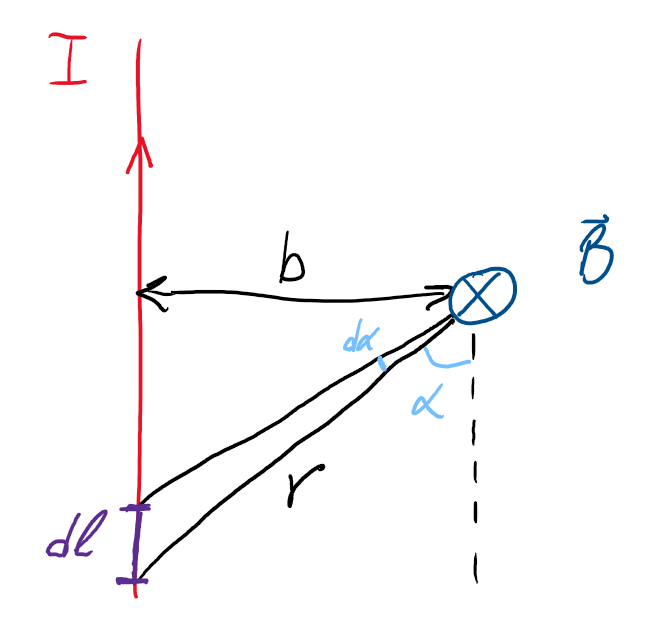
\includegraphics[width=5.8cm]{physics2/images/physics2_2025_02_10_2}
    \end{wrapfigure}

    \Ex Магнитное поле прямого тока, то есть тока, текущего по тонкому прямому проводу. Согласно формуле в произвольной точке $A$
    векторы $dB$ от всех элементов тока имеют одинаковое направление. Поэтому сложение векторов $dB$ можно заменить сложением 
    их модулей: $dB = \frac{Idl \cdot r \sin \alpha}{r^3} = \frac{\mu_0}{4\pi} I \frac{dl \sin\alpha}{r^2} =
    \frac{\mu_0}{4\pi} I \frac{r d\alpha}{r^2} = \frac{\mu_0}{4\pi} I \frac{d\alpha}{\frac{b}{\sin\alpha}} = \frac{\mu_0}{4\pi} \frac{I}{b} \sin \alpha d\alpha$, где $b$ - расстояние от точки до прямого проводника

    В интеграле получаем $B = \frac{\mu_0}{4\pi} \int_{0}^{\pi} \frac{I}{b} \sin \alpha d\alpha = \frac{\mu_0}{4\pi} \frac{I}{b} (\cos \alpha_1 - \cos \alpha_2)$

    Для бесконечного проводника получаем $B = \frac{\mu_0}{2\pi} \frac{I}{b}$
\end{minipage}

Линии магнитной индукции поля прямого тока представляют собой систему охватывающих провод концентрических окружностей

\begin{center}
    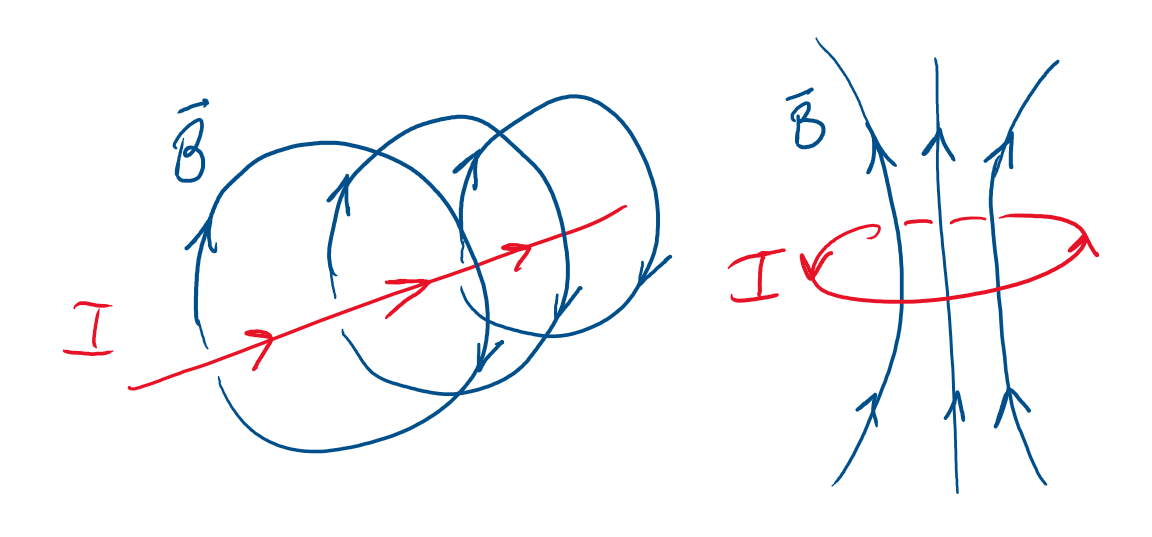
\includegraphics[width=0.7\textwidth]{physics2/images/physics2_2025_02_10_1}
\end{center}

Важно заметить, что линии электрического поля не замкнуты - у них есть начало (в плюсе) и конец (в минус), тогда 
как линии магнитного поля - замкнуты

\begin{minipage}{\textwidth}
    \begin{wrapfigure}{R}{0pt}
        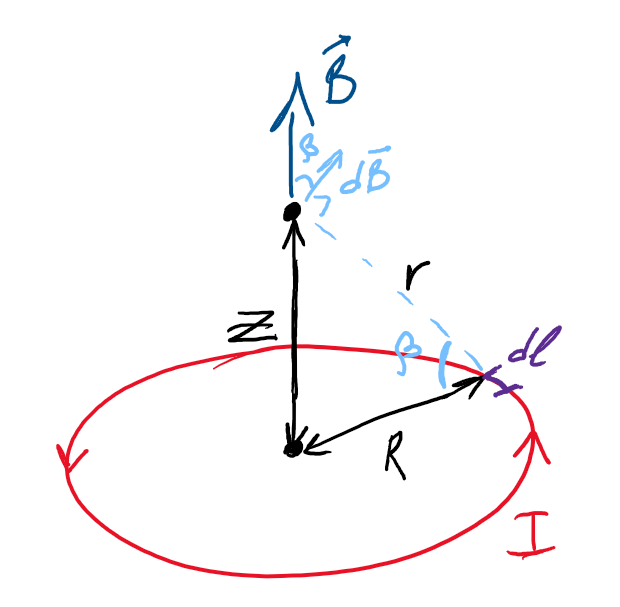
\includegraphics[width=5.8cm]{physics2/images/physics2_2025_02_10_3}
    \end{wrapfigure}

    \Ex Магнитное поле на оси кругового тока. Ищем вектор индукции в точке на оси кольца. 
    В силу симметрии вектор магнитной индукции сонаправлен оси кольца. По закону Био-Савара получаем

    $dB_z = dB \cos \beta = \frac{\mu_0}{4\pi} \frac{Idl \cdot r\sin 90^\circ}{r^3} \cos \beta$

    $\cos \beta = \frac{R}{r} \Longrightarrow B(z) = \frac{\mu_0}{4\pi} \frac{2\pi R^2 I}{(z^2 + R^2)^\frac{3}{2}} = \frac{\mu_0 R^2 I}{2 (z^2 + R^2)^\frac{3}{2}}$
\end{minipage}


